http://www.geomerics.com/blogs/demystifying-the-enlighten-precompute/


\chapter{Radiosity}\label{chp:radiosity}
Path tracing is an elegant and accurate global illumination algorithm, which handles almost all types of light paths, such as reflection, specular, caustics, etc. The most disadvantage of path tracing is that it is view dependent, which means that we need to recompute the whole image once the camera moved. And that makes it is not suitable for games, because most of the time, the characters are moving, the leaves are animating, and the mountain is closing, etc. On the other hand, diffuse lighting, which reflect lights all the same in every direction, is view-independent and so can be precomputed in advance. 

In 3D computer graphics, \textit{radiosity} is an application of the \textit{finite element method} to solve the rendering equation for scenes with surfaces that reflect light diffusely. Unlike path tracing, it only accounts for paths (represented by code "$LD^{*}E$") which leave a light source and are reflected diffusely some number of times (possibly zero) before hitting the eye. Radiosity methods were first developed in about 1950 in the engineering field of heat transfer. And it has been introduced into computer graphics field in 1984\cite[-14mm]{a:ModelingtheInteractionofLightBetweenDiffuseSurfaces} by researchers at Cornell University and Hiroshima University.

Due to it can be precomputed and so satisfy the real-time needs for games. The most notable commercial radiosity middleware Enlightn\footnote{\url{http://www.geomerics.com/enlighten/}}, by Geomerics has been adopted by several games including Battlefield 3 and Need for Speed: The Run. It even has been built in the Unity3D\footnote{\url{http://blogs.unity3d.com/2014/09/18/global-illumination-in-unity-5/}} engine.




\section{Basis}
Let's start with the derivation of the radiosity system of linear equations.


\subsection{The Radiosity System of Linear Equations}
Let's recall the rendering equation:

\begin{equation*}
	L(x\to\Theta)=L_e(x\to\Theta)+\int_{\Omega_x}f_r(x,\Theta^{'}\to\Theta)L(x\leftarrow\Theta^{'})cos(N_x,\Theta^{'})d\omega_{\Theta^{'}}
\end{equation*}

On purely diffuse surface, see figure \ref{f:radiosity-diffuse}, self-emitted radiance $L_e(x)$ and the BRDF $f_r(x)$ do not depend on directions $\Theta$ and $\Theta^{'}$. The rendering equation then becomes:

\begin{figure}
\sidecaption
	\includegraphics[width=0.65\textwidth]{graphics/gi/path-23}
	\caption{For radiosity, the key assumption is that all surfaces are ideal diffuse (Lambertian) reflectors.}
	\label{f:radiosity-diffuse}
\end{figure}

\begin{equation*}
	L(x)=L_e(x)+\int_{\Omega_x}f_r(x)L(x\leftarrow\Theta^{'})cos(N_x,\Theta^{'})d\omega_{\Theta^{'}}
\end{equation*}

The incident radiance $L(x\leftarrow\Theta^{'})$ still depends on incident direction, which corresponds to the exitant radiance $L(y)$ emitted towards $x$ by the point $y$ visible from $x$ along the direction $\Theta^{'}$, see figure \ref{f:The-geometry-of-the-surfaces}. As explained in section \ref{sec:surface-form}, the integral above, over the hemisphere $\Omega_x$, can be transformed into an integral over all surfaces $S$ in the scene (equation \ref{e:integral-over-area}). The result is an integral equation in which no directions appear anymore:

\begin{figure}
\sidecaption
	\includegraphics[width=0.65\textwidth]{graphics/gi/path-18}
	\caption{The geometry of the surfaces.}
	\label{f:The-geometry-of-the-surfaces}
\end{figure}

\begin{equation*}
	L(x)=L_e(x)+\rho(x)\int_{S}K(x,y)L(y)dA_y
\end{equation*}

In a diffuse environment, radiosity and radiance are related as $B(x)=\pi L(x)$ and $B_e(x)=\pi L_e(x)$. Multiplication by $\pi$ of the left- and right-hand sides of the above equation yields the \textit{radiosity integral equation}:

\begin{equation}\label{e:radiosity-integral-equatoin}
	B(x)=B_e(x)+\rho(x)\int_S K(x,y)B(y)dA_y
\end{equation}

The kernel of this integral equation is:

\begin{equation*}
\begin{aligned}
	K(x,y)&=G(x,y)V(x,y) \text{, with }\\
		G(x,y)&=\frac{cos(\Theta_{xy},N_x)cos(-\Theta_{xy},N_y)}{\pi r^{2}_{xy}}
\end{aligned}
\end{equation*}

$\Theta_{xy}$ is the direction pointing from $x$ to $y$. $r^{2}_{xy}$ is the square distance between $x$ and $y$. $V(x,y)$ is the visibility predicate ($1$ if $x$ and $y$ are mutually visible, $0$ otherwise).

The \textit{average radiosity} $B_i$ emitted by a surface patch $i$ with area $A_i$ is then:

\begin{equation}\label{e:average-radiosity}
	\begin{aligned}
		B_i&=\frac{1}{A_i}\int_{S_i} \int_{\Omega_x} L(x\to\Theta)cos(\Theta,N_x)d\omega_\Theta dA_x\\
		   &=\frac{1}{A_i}\int_{S_i}L(x) \int_{\Omega_x} cos(\Theta,N_x)d\omega_\Theta dA_x\\
		   &=\frac{1}{A_i}\int_{S_i}L(x)\pi dA_x\\
		   &=\frac{1}{A_i}\int_{S_i}B(x)dA_x
	\end{aligned}
\end{equation}

Let's assume the radiosity $B(x)$ is constant on each patch $i$, $B(x)=B^{'}_{i},x\in S_i$. Equation \ref{e:radiosity-integral-equatoin} can be converted into a linear system as follows:

\begin{equation*}
\begin{aligned}
	B_{i}^{'}=&B_i=\frac{1}{A_i}\int_{S_i}B(x)dA_x\\
			 =&\frac{1}{A_i}\int_{S_i}B_e(x)dA_x+\frac{1}{A_i}\int_{S_i}\int_S \rho (x)K(x,y)B(y)dA_ydA_x\\	
			 =&\frac{1}{A_i}\int_{S_i}B_e(x)dA_x+\sum_j \frac{1}{A_i}\int_{S_i}\int_{S_j} \rho (x)K(x,y)B(y)dA_ydA_x\\
			 =&B_{ei}+\sum_j B_{j}^{'}\frac{1}{A_i}\int_{S_i}\int_{S_j} \rho (x)K(x,y)dA_ydA_x
\end{aligned}
\end{equation*}

If we now also assume that the reflectivity is constant over each patch $\rho(x)=\rho_i,x\in S_i$, the following classical \textit{radiosity system of equations} results:

\begin{equation}\label{e:radiosity-system-of-equations}
	B_{i}^{'}=B_{ei}+\rho_i\sum_j F_{ij}B^{'}_{j}
\end{equation}

The factors $F_{ij}$ are called \textit{patch-to-patch form factors}, which we will discuss later:

\begin{equation}
	F_{ij}=\frac{1}{A_i}\int_{S_i}\int_{S_j}K(x,y)dA_ydA_x
\end{equation}

Note that the radiosities $B^{'}_{i}$ that result after solving the system of linear equations (equation \ref{e:radiosity-system-of-equations}) are only an approximation for the average radiosities (equation \ref{e:average-radiosity}). The true radiosity $B(y)$, which was replaced by $B^{'}_j$ in the equations above, is in practice only very rarely piecewise constant! The difference between $B_{i}$ and $B_{i}^{'}$ is, however, rarely visible in practice. For this reason, we will denote both the average radiosity $B_{i}$ and he radiosity coefficients $B_{i}^{'}$ by $B_{i}$. 



\subsection{Explanation of $B_i$}
Confused? Don't worry, let's get it clear. Sometimes we learn computer graphics concepts by combining the mathematics and conclusions.

First and the most important, for radiosity, the key assumption is that all surfaces are ideal diffuse (Lambertian) reflectors. For diffuse lighting, the most useful feature is that it is independent of observer position, and thus environments can be preprocessed for dynamic sequences.

So to precompute some kind of quantity, we need to get rid of the directions in the rendering equation. We figure out radiosity $B(x)$ is the quantity that we need. In the radiosity integral equation \ref{e:radiosity-integral-equatoin}, the radiosity $B(x)$ of a point $x$ is depend on all the other radiosity $B(y)$ in the scene $S$ and the $K(x,y)$. They are both change slowly within a small area, a patch. So we can use an average radiosity $B_i$ approximate the true radiosity $B(x)$. That, conversely, needs a small enough patch, in which the radiosity $B(x)$ is approximately constant.

\begin{figure}\label{f:radiosity-system-of-equations}
	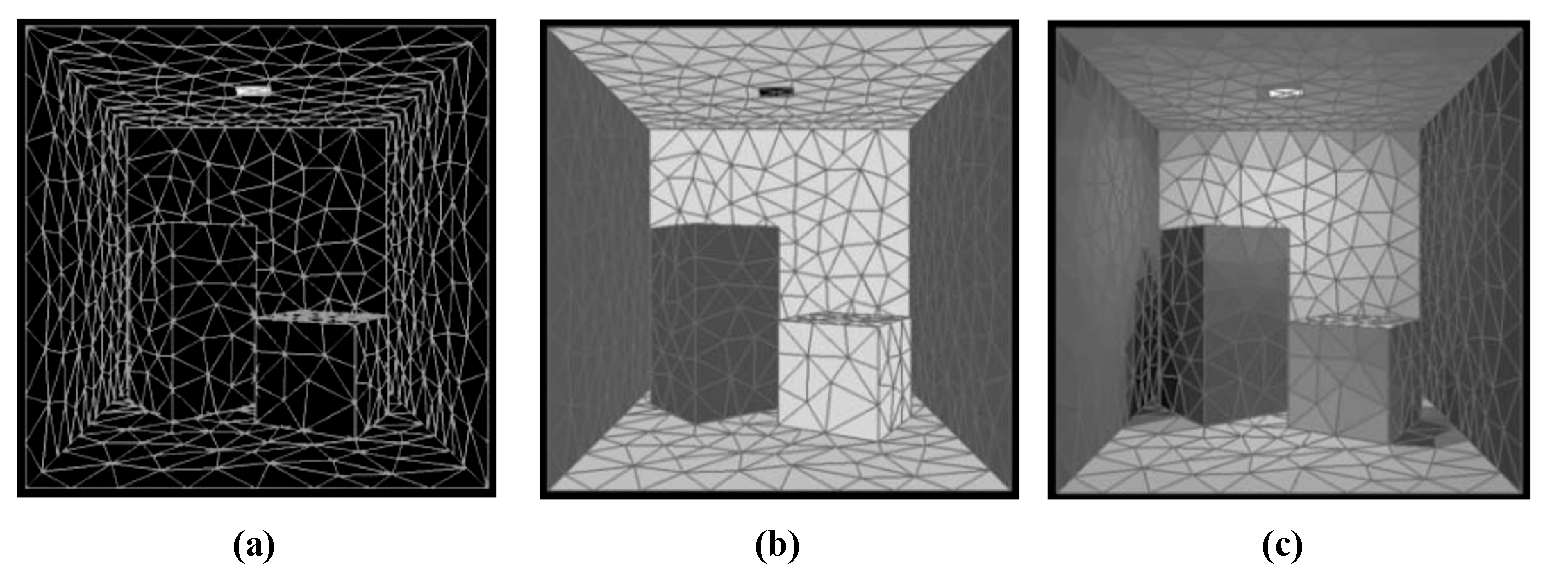
\includegraphics[width=1.0\textwidth]{graphics/gi/path-19}
	\caption{The input of the classic radiosity method consists of a list of patches (triangles, in this example) with their average self-emitted radiosity $B_{i}^{e}$ (left) and reflectivity $\rho_i$ (middle) given. These data suffice in order to compute the average total radiosities $B_i$ (right), including the effect of light bouncing around. The computed radiosities are converted to display colors for each patch. The resulting, "illuminated," model can be rendered from any viewpoint, at interactive rates using graphics hardware.}
\end{figure}

Within a small patch, the reflectance is change slowly thus can also be approximately constant $\rho_i$. So we derive the radiosity system of equations, depicted in figure \ref{f:radiosity-system-of-equations}.

The classic radiosity method is an instance of a larger class of numerical methods called \textit{finite element methods} (EFM), which is a numerical technique for finding approximate solutions to boundary value problems for partial differential equations. It uses subdivision of a whole problem domain into simpler parts, called finite elements, and variational methods from the calculus of variations to solve the problem by minimizing an associated error function. Analogous to the idea that connecting many tiny straight lines can approximate a larger circle, FEM encompasses methods for connecting many simple element equations over many small subdomains, named finite elements, to approximate a more complex equation over a larger domain.   

From the radiosity system of equations (equation \ref{e:radiosity-system-of-equations}), we can conclude the steps of the classic radiosity method:

\begin{figure}
\sidecaption
	\includegraphics[width=0.65\textwidth]{graphics/gi/path-24}
	\caption{Discretization of the input geometry into patches.}
	\label{f:Discretization}
\end{figure}

\begin{enumerate}
	\item  Discretization (figure \ref{f:Discretization}) of the input geometry into patches $i$.
	\item Computation of form factors $F_{ij}$, for every pair of patches $i$ and $j$.
	\item Numerical solution of the radiosity system of linear equations.
	\item Display of the solution, including the transformation of the resulting radiosity values $B_i$ (one for each patch and considered wavelength) to display colors.  
\end{enumerate}



\section{The Form Factors}
The form factor $F_{ij}$, which is also called \textit{geometrical view factor} \footnote{\url{https://en.wikipedia.org/wiki/View\_factor}} in radiative heat transfer, indicates what fraction of the irradiance on $i$ originates at $j$. 

In the game field, the form factors usually has been precomputed in advance, so the materials and light sources can change dynamically in runtime. The radiosity system of linear equation needs to be solved at runtime. We'll discuss more details in section \ref{sec:enlighten}. So radiosities usually is used to describe a static scene. But we'll also discuss some methods are used to handle dynamic objects in the scene with radiosity in section \ref{sec:dynamic-radiosity}. 

Form factors have the following properties:

\begin{itemize}
	\item The form factors are all positive or zero in a scene consisting of closed, opaque objects: they cannot be negative because the integrand is positive or zero. They will be equal to zero for a pair of patches i and j that are mutually invisible.
	\item The form factors $F_{ij}$ between a patch $i$ and all other patches $j$ in a scene sum to at most one:
	
		\begin{equation*}
			\sum_j F_{ij}\begin{cases}
				  =1  & \text{if the scene is closed}\\
			      <1  & \text{otherwise } 
				\end{cases}
		\end{equation*}
	\item The form factors satisfy the following \textit{reciprocity relation}:
		\begin{equation*}
			A_iF_{ij}=A_jF_{ji}
		\end{equation*}
\end{itemize}




\subsection{The HEMI-CUBE}\label{sec:the-hemi-cube}
It's been proven that it's difficult to solve the double area integral of the form factor analytically. A more general approach is needed to handle this integral. 

If the distance between the two patches is large compared to their size, and they are not partially occluded from one another. It can be seen that the integrand of the inner integral remains almost constant. In that case the effect of the outer integral is simply a multiplication by one and finding a solution to the inner integral will provide a good approximation for the form-factor:

\begin{equation}\label{e:single-integral}
	F_{ij}\approx F_{\delta ij}=\int_{S_j}\frac{cos\Theta_x cos\Theta_y}{\pi r^{2}_{xy}} HID dA_j
\end{equation}

where HID function incorporates the occlusion between surfaces by returning zero or one depending on the presence of an occluding object between the points on the surfaces. If the patches are close together relative to their size, or there is partial occlusion, the patches can be subdivided into smaller patches and the single integral equation approximation can still be used.

\begin{figure}
\sidecaption
	\includegraphics[width=0.65\textwidth]{graphics/gi/path-20}
	\caption{The geometrical form factor (or "projected solid angle") $F_{ij}$. }
	\label{f:hemispherical}
\end{figure}

A geometry analog for the single form-factor integral was developed by Wilhelm Nusselt, and is called the \textit{Nusselt analog}, see figure \ref{f:hemispherical}. For a finite area, the form-factor is equivalent to the fraction of the circle (which is the base of the hemisphere) covered by projecting the area onto the hemisphere and then orthographically down onto the circle.

\begin{figure}\label{f:hemicube}
	\begin{subfigure}[b]{0.54\textwidth}
		\includegraphics[width=1.0\textwidth]{graphics/gi/path-22-1}
	\end{subfigure}
	\begin{subfigure}[b]{0.45\textwidth}
		\includegraphics[width=1.0\textwidth]{graphics/gi/path-22-2}
	\end{subfigure}
	\caption{Left:) Areas with identical form-factor; Right:) The HEMI-CUBE.}
\end{figure}

From the definition of the form-factor it can be seen that any two patches in the environment, which when projected onto the hemisphere occupy the same area and location, will have the same form-factor value. This is also true for projections onto any other surrounding surface, see figure \ref{f:hemicube}(Left).

Projecting to a curved surface such as a hemisphere is complex. Instead of projecting onto a sphere, Cohen and Greenberg \cite{a:Thehemi-cube:aradiositysolutionforcomplexenvironments} constructs an imaginary cube around the center of the receiving patch, see figure \ref{f:hemicube}(Right). These faces of the cube are divided into square "pixels" at a given resolution, generally between $50\times 50$ and $100\times 100$, and the environment is then projected onto the five planar surfaces.

The projection to the hemicube is done using rasterization, and a depth buffer is used to determine which patch is "seen " in that particular direction by comparing distances to each patch and selecting the nearer one. 

A specific \textit{delta form-factor} value for each pixel on the cube is found for the differential area to differential area form-factor and stored in a lookup table, This table need only contain values for one eighth of the top face and one quarter of one side face due to symmetry.



\subsection{Sampling Approaches}
We can also use sampling approaches to solve the radiosity system of linear equations.

The interpretation of a form factor being the fraction of power emitted by a first patch $i$ that lands on a second patch $j$ immediately suggests that form factors can be estimated by means of a very simple and straightforward simulation: Let $i$ be the source of a number $N_i$ of virtual particles that behave like photons originating on a diffuse surface. The number $N_{ij}$ of these particles that land on the second patch $j$ yields an estimate for the form factor: $N_{ij}/N_i\approx F_{ij}$. See figure \ref{f:sampling-methods} (Left).

Consider a particle originating at a uniformly chose location $x$ on $S_i$ and being shot into a cosine-distributed direction $\Theta$ with regard to the surface normal $N_x$ at $x$. The probability density $p(x,\Theta)$ associated with such a particle is:

\begin{equation*}
	p(x,\Theta)=\frac{1}{A_i} \times \frac{cos(\Theta,N_x)}{\pi}
\end{equation*}

Now, let $\chi_i(x,\Theta)$ be a predicate taking value $1$ or $0$ depending on whether or not the ray shot from $x$ into $\Theta$ hits a second patch $j$. The probability $P_{ij}$ that such a ray lands on a second patch $j$ then is:

\begin{equation*}
\begin{aligned}
	P_{ij}=&\int_{S_i}\int_{\Omega_x}\chi_j(x,\Theta)p(x,\Theta)dA_xd\omega_\Theta\\
	=&\int_{S_i}\int_S \chi_j(x,\Theta)\frac{1}{A_i} \frac{cos(\Theta_{xy},N_x)cos(-\Theta_{xy},N_x)}{\pi r^{2}_{xy}} V(x,y)dA_y dA_x\\
	=&\frac{1}{A_i}\int_{S_i}\int_S\frac{cos(\Theta_{xy},N_x)cos(-\Theta_{xy},N_x)}{\pi r^{2}_{xy}} V(x,y)dA_y dA_x\\
	=&F_{ij}
\end{aligned}
\end{equation*}

When shooting $N_i$ such particles from $i$, the expected number of hits on patch $j$ will be $N_iF_{ij}$. This method of estimating form factors was proposed at the end of the 1980s as a ray-tracing alternative for the hemicube algorithm for form factor computation \cite[-16mm]{a:AGeneralTwo-PassMethodIntegratingSpecularandDiffuseReflection} \cite[2mm]{a:ARayTracingMethodforIlluminationCalculationinDiffuse-SpecularScenes}. 

The algorithm of the previous section requires us to shoot so-called local lines: lines with an origin and direction selected with regard to a particular patch i in the scene. There exist, however, a number of algorithms for form factor sampling based on \textit{uniformly distributed global} lines, see figure \ref{f:sampling-methods}(Right). Several such sampling algorithms have been proposed for use with radiosity, for instance \cite[-12mm]{a:TheUseofGlobalRandomDirectionstoComputeRadiosityGlobalMonteCarloTechniques}. 

\begin{figure}\label{f:sampling-methods}
	\begin{subfigure}[b]{0.5\textwidth}
		\includegraphics[width=1.0\textwidth]{graphics/gi/path-21-1}
	\end{subfigure}
	\begin{subfigure}[b]{0.5\textwidth}
		\includegraphics[width=1.0\textwidth]{graphics/gi/path-21-2}
	\end{subfigure}
	\caption{Form factor sampling: (Left) The fraction of local lines hitting a particular destination patch is an estimate for the form factor between source and destination. Global lines (right) are constructed without reference to any of the patches in the scene.}
\end{figure}

The fact that form factors are probabilities that can be sampled efficiently leads to algorithms that allow us to solve the radiosity system of equations without the need to ever compute the value of a form factor. You can cheek more details about this called \textit{stochastic radiosity} methods in the book \cite{b:AdvancedGlobalIllumination} in section $6.3$ and $6.4$. But due to it is more simple and friendly to rasterization, hemicube is more common especially when it runs on GPU.




\section{Enlighten}\label{sec:enlighten}
Enlighten\footnote{\url{http://www.geomerics.com/enlighten/}}, by Geomerics themselves, "is the industry's most advanced dynamic lighting technology, delivering real-time global illumination across all gaming platforms."

\begin{figure}
	\includegraphics[width=1.0\textwidth]{graphics/gi/path-25}
	\caption{Image rendered by using Enlighten (Image courtesy of Geomerics).}
\end{figure}

Inside Enlighten, the core is the radiosity algorithm, which provides indirect diffuse lighting for the game. With some other approaches, Enlighten also support dynamic specular reflections, dynamic objects, etc. Enlighten is a middleware radiosity package which can be integrated with your own renderer or the third part famous game engine such as Unreal Engine 4 and it's been built in Unity 5\footnote{\url{http://blogs.unity3d.com/2014/09/18/global-illumination-in-unity-5/}}.

Basically, using Enlighten involves two phases: first precompute the surface-to-surface visibility of static geometry in the scene, and at runtime Enlighten uses these data to generate some output data which will be used by the renderer. A good material about Enlighten architecture can be found in \cite[-10mm]{a:AReal-TimeRadiosityArchitectureforVideoGame}.



\subsection{Precomputation}
During the precomputation phase, see figure \ref{f:enlighten-precompute}, Enlighten will decompose scene into system,  compute the form factors and compute the lightmap uvs. These output data will be used to compute lightmaps and lightprobes at runtime.

\begin{figure}\label{f:enlighten-precompute}
	\begin{center}
		\includegraphics[width=0.8\textwidth]{graphics/gi/path-29-1}
	\end{center}
	\caption{Enlighten precompute phase.}
\end{figure}

First, Enlighten will automatically break up the scene into \textit{systems}, see figure \ref{f:systems}(a). A system is a collection of meshes that can be processed independently, and thus each system can be processed in parallel. Each system outputs a small lightmap for part of the scene.

\begin{figure*}\label{f:systems}
	\begin{subfigure}[b]{0.285\textwidth}
		\includegraphics[width=1.0\textwidth]{graphics/gi/path-30-1}
		\caption{Systems}
	\end{subfigure}
	\begin{subfigure}[b]{0.285\textwidth}
		\includegraphics[width=1.0\textwidth]{graphics/gi/path-30-2}
		\caption{Input dependencies}
	\end{subfigure}
	\begin{subfigure}[b]{0.42\textwidth}
		\includegraphics[width=1.0\textwidth]{graphics/gi/path-30-3}
		\caption{System atlases}
	\end{subfigure}
	\caption{Radiosity systems. Note that systems are not the patches of radiosity which are used to compute form factors.}
\end{figure*}

Enlighten also automatically define input dependencies (see figure \ref{f:systems}(b)) to each system, which is a way to put restrictions on the light transport. So when we update the yellow system here, we only read bounce light from the green systems and we can forget about the rest.

Systems are also used to control update performance. Large systems will have many pixels and it will take longer to compute, so by creating many small systems, it can spread out radiosity updates on seversal frames if. It typically update one system per CPU core every frame.

And lastly, Enlighten pack a uv atlas for each system, see figure \ref{f:systems}(c). Each system atlas is independent of all other systems, so it ends up with one lightmap per system.



\subsection{Rendering}
The main runtime operation in Enlighten is to map a point sampled description of the lighting over the target mesh surface, to\footnote{\url{http://www.geomerics.com/blogs/enlighten-output/}}:

\begin{itemize}
	\item Lightmaps
	\item Light probes (spherical harmonics)
	\item Cubemaps
\end{itemize}

This is the bounce. Anything you can express in these terms is valid input to Enlighten. Such as environment light, area lights, or some other type of lighting incident on your geometry surface which can be point sampled. Even the previous lightmap output can be fed to Enlighten as an input light to generate a second bounce. This is how Enlighten generate multiple bounces. In Enlighten, only one iteration of radiosity propagation is executed per frame. Multiple light bounces are simulated by using the previous frame as light input for the computation.
 
 \begin{figure}\label{f:enlighten-precompute}
	\begin{center}
		\includegraphics[width=0.9\textwidth]{graphics/gi/path-29-2}
	\end{center}
	\caption{Enlighten runtime phase.}
\end{figure}

Because Enlighten only precompute geometry information, and the above output datas are generated at runtime. So Enlighten allows dynamically changing:

\begin{itemize}
	\item Light sources.
	\item Environment lighting.
	\item Material properties (diffuse reflectivity and surface emission).
\end{itemize}

\begin{figure}
\sidecaption
	\includegraphics[width=0.65\textwidth]{graphics/gi/path-27}
	\caption{The light probe configuration for Realistic Room (Image courtesy of Geomerics).}
	\label{f:enlighten-light-probe}
\end{figure}

Because the key for radiosity is to precompute surface-to-surface visibility, so the geometry that is part of the global illumination has to be static. But dynamic geometry can be relit using light probes (see figure \ref{f:enlighten-light-probe}) that are updated in real-time with the global illumination generated from the static geometry. The main limitations is: dynamic geometry conot bounce or emit light into the global illumination solution. So the dynamic objects need to be small, because smaller objects normally do not contribute much to the global illumination.

However, recently, significant new feature has been added in  Enlighten: Dynamic objects contributing to radiosity, suitable for large dynamic occluders in a scene, not suitable or necessary for small dynamic objects.

We will detail light probes technique in future chapters.



\subsection{Radiosity Intepolation}
To render an image the discretzied radiosity information is used to create a continuous shading across a given surface (or polygon). 

A simple method\footnote{Note: We don't know what interpolation method Enlighten has adopted. This is just a common method.} uses a bilinear interpolation within each patch. This bilinear variation of radiosities insures first order continuity at patch edges. In order to perform the interpolation, radiosity values must be transferred from the patches themselves to each vertex of the patches. See figure \ref{f:vertex-radiosities}.

For each polygon, the radiosities of patch vertices which are interior to the polygon containing the patch are computed as the average of radiosities of the surrounding patches. Exterior vertex radiosities are extrapolated values from the adjacent interior vertex radiosities through an average of the adjacent patch radiosities. Finally, the resulting vertex radiosities are used for the bilinear interpolation within each patch. See figure \ref{f:vertex-radiosities}.

\begin{figure}\label{f:vertex-radiosities}
	\begin{center}
		\includegraphics[width=0.7\textwidth]{graphics/gi/path-34}
	\end{center}
	\caption{Patch radiosities $\to$ vertex radiosities}
\end{figure}

In Enlighten, the discretzied mesh is called \textit{target mesh} (which equals patches). Figure \ref{f:enlighten-output}(Left) is what the previous point sampled data is mapped to. In some scene, this is the raw lightmap output from Enlighten, before any interpolation, albedo modulation or directional relighting is applied.

\begin{figure*}\label{f:enlighten-output}
	\begin{subfigure}[b]{0.5\textwidth}
		\includegraphics[width=1.0\textwidth]{graphics/gi/path-29-6}
	\end{subfigure}
	\begin{subfigure}[b]{0.5\textwidth}
		\includegraphics[width=1.0\textwidth]{graphics/gi/path-29-7}
	\end{subfigure}
	\caption{Enlighten output. Left:)Target; Right:)Detail (Image courtesy of Geomerics).}
\end{figure*}

Figure \ref{f:enlighten-output}(Right) shows exactly the same lighting data, but applied to the detailed geometry, together  with normal maps and indirect specular.



\subsection{Dynamic Reflections}
Due to radiosity theory assumes all the surfaces are diffusely, so it cannot include specular effect. But it is well known that reflections and shadows are key topics in any game. Without reflections and shadows any virtual world would look plain and unrealistic. 

For reflection effect, it can be implemented by rendering a "environment" texture( see figure \ref{f:reflection-case}(Left)) into the specular surfaces, of course the reflectance of the surface will blur the reflection (see figure \ref{f:reflection-case}(Right)).

\begin{figure}\label{f:reflection-case}
	\includegraphics[width=1.0\textwidth]{graphics/gi/path-31}
	\caption{Reflections on the corridor at the Taiwan Taoyuan International Airport.}
\end{figure}

Based on this observation, cube maps\cite{a:EnvironmentMappingandOtherApplicationsofWorldProjections} are typically used to create reflections from an environment that is considered to be infinitely far away. But with a small amount of shader math, we can place objects inside a reflection environment of a specific size and location, providing higher quality, image-based lighting (IBL).

One aspect of such reflections defies realism: the reflection from a cube map always appears as if it's infinitely far away. This limits the usefulness of cube maps for small, enclosed environments. When moving models through an interior environment, it would be useful to have a cube map that behaved as if it were only a short distance away-say, as big as the current room. As the model moved within that room, the reflections would scale appropriately bigger or smaller, according to the model's location in the room, see figure \ref{f:reflection-error}.

\begin{figure}\label{f:reflection-error}
	\begin{subfigure}[b]{0.5\textwidth}
		\includegraphics[width=1.0\textwidth]{graphics/gi/path-32-1}
	\end{subfigure}
	\begin{subfigure}[b]{0.5\textwidth}
		\includegraphics[width=1.0\textwidth]{graphics/gi/path-32-2}
	\end{subfigure}
	\caption{Left:)Reflective Object with Localized Reflection; Right:)Localized Reflection in a Different Location.}
\end{figure}

Local cube map is the technique which added a local correction to reflections based on cube maps. The solution to this problem was first proposed by Kevin Bjorke\footnote{\url{http://http.developer.nvidia.com/GPUGems/gpugems_ch19.html}} in 2004, see figure \ref{f:reflection-local}(Left). A few years later, in 2010, a better solution was proposed\footnote{\url{http://www.gamedev.net/topic/568829-box-projected-cubemap-environment-mapping/?&p=4637262}} in a thread of a developer forum at gamedev.net. The new approach replaced the previous bounding sphere by a box, solving the shortcomings of Bjorke's method: deformations and complexity of the algorithm to find the intersection point, see figure \ref{f:reflection-local}(Right). More details can be found in \footnote{\url{https://seblagarde.wordpress.com/2012/09/29/image-based-lighting-approaches-and-parallax-corrected-cubemap/}}.

Enlighten reflection captures are used for efficient, per-pixel directional look-up for reflections which can be used on either moving objects or static geometry.  Each reflection capture is a cube map which encodes the view of the scene in all directions and contains the incoming light at the position of the reflection capture. They provide input for physically based shading via the roughness parameter, which can be used to control how much a reflection is blurred depending on the surface material.

\begin{figure}\label{f:reflection-local}
	\begin{subfigure}[b]{0.59\textwidth}
		\includegraphics[width=1.0\textwidth]{graphics/gi/path-33-1}
	\end{subfigure}
	\begin{subfigure}[b]{0.39\textwidth}
		\includegraphics[width=1.0\textwidth]{graphics/gi/path-33-2}
	\end{subfigure}
	\caption{Left:)Reflections using local cubemaps; Right:)Introducing a bounding box.}
\end{figure}

Reflection captures are authored manually throughout the scene and require extra data for rendering. For example a box can be added to enable box projection when shading shiny objects: the view ray will bounce off in a certain direction and the position at which this intersects the box will determine where to look up the correct values in the cube map to shade the object.

\begin{figure}
	\includegraphics[width=1.0\textwidth]{graphics/gi/path-28}
	\caption{A reflection capture in Realistic Room with extra data for box projection (Image courtesy of Geomerics).}
\end{figure}





\section{Real-Time Dynamic Radiosity}\label{sec:dynamic-radiosity}
Radiosity is an semi-precompute technique for global illumination. It guarantees high quality and also better performance than path tracing. With some optimization, Enlighten can even reach real-time performance and has been proven  by some famous titles. 

Although radiosity is designed for static scenes, since it was born, many smart engineers have proposed several approaches which try to work with dynamic scenes. Until 2013, the called \textit{cross redistribution radiosity} has acquired its first descendant technique which combines high image quality with real-time results. 

These algorithms and methods also have shown a good philosophy, I think, for real-time rendering: they try to recompute the only part of the whole computation has changed since last frame, and they try best to utilize the geometry coherence of the scenes.




\subsection{Progressive Refinement Radiosity}
Recall the classical radiosity system of equations:

\begin{equation}\label{e:radiosity-equation}
	B_i=B_{ei}+\rho_i \sum_j F_{ij} B_j
\end{equation}

If we want to get the value of $B_i$, we need to know all other $B_j$, thus we must solve the whole radiosity system of equations. And only if we've solved the equations, we then could show the result image to the user. This method cannot satisfy the need of interactive manipulation. 

One approach to accommodating the competing demands of interactivity and image quality is offered by the method of rendering by adaptive refinement\cite[-5mm]{a:ImageRenderingbyAdaptiveRefinement}. In the words of Bergman, what is needed is a \textit{golden thread}, a single rendering operation that, with repeated application, will continually refine the quality of an image. In 1988, Michael F. Cohen, et al., presented\cite{a:AProgressiveRefinementApproachtoFastRadiosityImageGeneration} a reformulation of the radiosity algorithm that provides such a thread.

In equation \ref{e:radiosity-equation}, the lighting leaving patch $i$ is determined by \textit{gathering} in the light from the rest of the environment, see figure \ref{f:gathering-and-shooting}(a). A single term from the summation in equation \ref{e:radiosity-equation} determines the contribution to the radiosity of patch $i$ from patch $j$:

\begin{equation*}
	B_i \text{ due to }B_j=\rho_i B_j F_{ij}
\end{equation*}

\begin{figure}
	\begin{subfigure}[b]{.48\textwidth}
		\includegraphics[width=1.\textwidth]{graphics/gi/path-35-1}
		\caption{Gathering}
	\end{subfigure}
	\begin{subfigure}[b]{.48\textwidth}
		\includegraphics[width=1.\textwidth]{graphics/gi/path-35-2}
		\caption{Shooting}
	\end{subfigure}
	\caption{Gathering vs. Shooting}	
	\label{f:gathering-and-shooting}
\end{figure}

It is possible to reverse this process by determining the contribution made by patch $i$ to the radiosity of all other patches. The reciprocity relationship provides the basis for reversing this relationship. The contribution of the radiosity from patch $i$ to the radiosity of patch $j$ is:

\begin{equation}
	B_j\text{ due to }B_i=\rho_j B_iF_{ij}A_i/A_j
\end{equation}

This is true for all patches $j$. Thus the total contribution to an environment from the radiosity of patch $i$ is given by:

\begin{equation}
	\text{For all patches $j$ : $B_j$ due to $B_i=\rho_jB_iF_{ij}A_i/A_j$}
\end{equation}

Note the form-factors are still calculated using the hemi-cube placed at patch $i$. Thus, each step of the solution now consists of performing a single hemi-cube over a patch and adding the contribution from the radiosity of that patch to the radiosities of all other patches, in effect, \textit{shooting} light out from that patch into the environment, see figure \ref{f:gathering-and-shooting}(b). Since only the form-factors from the shooting patches are needed, the form-factors can be computed on-the-fly after each shooting patch is found.

During the course of the iterative solution this step may be repeated for patch $i$ several times as the solution converges. Each time the estimate of the radiosity of patch $i$ will be more accurate. However, the environment will already include the contribution of the previous estimate of $B_i$. Thus, only the difference, $\triangle B_i$, between the previous and current estimates of $B_i$ needs to be considered. $\triangle B_i$ represents the unshot radiosity, see algorithm \ref{lst:progressive-refinement}.

\begin{lstlisting}[language=C++,mathescape,caption=Progressive refinement radiosity algorithm,label=lst:progressive-refinement]
for each iteration, for each patch $i$:
	calculate the form-factors $F_{ij}$ using a hemi-cube at patch $i$;
	for each patch $j$:
		$\triangle Rad = p_j\triangle B_iF_{ij}A_i/A_j$;
		$\triangle B_j = \triangle B_j + \triangle Rad$; /* update change since last time patch $j$ shot light */
		$B_i = B_j + \triangle Rad$; /* update total radiosity of patch $j$ */
	$\triangle B_i = 0$; /*reset unshot radiosity for patch $i$ to zero*/\end{lstlisting}

The above step continues until the solution converges to within the desired tolerance. Each intermediate step simultaneously improves the solution for many patches, providing intermediate results which can be displayed as the algorithm proceeds.

In addition to converging gracefully, it is desirable for the solution to improve in accuracy as quickly as possible. The algorithm is implemented by always shooting from the patch for which the difference, $\triangle B_iA_i$, between the previous and the current estimates of unshot radiant energy is greatest. Such as most light sources are automatically processed first by this rule, since initially all other patches will have a radiosity of zero.




\subsection{Incremental Radiosity}
The progressive refinement approach makes radiosity reach to interactive needs by reformulating the basic equation and rendering by progressive refinement. However, as with the other radiosity methods, this technique requires the rendered scene to be static. If any part of the scene is changed, the radiosity process will need to be repeated from scratch.

The \textit{incremental radiosity}\cite{a:IncrementalRadiosity:AnExtensionofProgressiveRadiositytoanInteractiveImageSynthesisSystem} is a new radiosity algorithm, which is an extension of progressive radiosity, to incrementally render scenes with changing geometry and surface attributes. The method supposes a modeling change generally exhibits some coherence and affects only parts of an image. It performs the radiosity computations incrementally based on the scene changes to reduce the rendering time.

This algorithm proceeds with the normal progressive solution. In the beginning of each solution cycle, though, the new method will monitor any requests from the user for scene changes. When a change is requested, the solution will be interrupted temporarily to process the request and resume when the processing is completed. The allowable changes currently include changing surface attributes, such as reflectance and emission, and scene geometry.



\subsubsection{Changing Surface Attributes}
When the attributes of a patch are changed, the patch's \textit{incremental radiosity} (the difference in radiosity as a result of the attribute change) is computed first. The incremental radiosity is then distributed in the same manner as distributing the unshot radiosity in the progressive refinement process.

The incremental radiosity of patch $i$, $\triangle B_i$, is:

\begin{equation}
	\triangle B_i=B^{'}_{ei}-B_{ei}+\frac{(\rho^{'}_i-\rho_i)(B_i-B_{ei})}{\rho_i}
\end{equation}

where $B^{'}_{ei}$ and $\rho^{'}_i$ is the new emission and reflectance of the patch $i$.


\subsubsection{Changing Scene Geometry}
Unlike attribute changes, geometry changes will modify some of the form-factors. Therefore, all the patches that have radiated energy to the scene need to reshoot their radiosities based on the form-factor changes. When a geometry change is made, every patch that has radiated energy is visited. For each of the patches, we need to first remove its radiosity contribution to the scene based on the old geometry, and then reshoot its total radiosity based on the new geometry.


\begin{figure*}
	\begin{subfigure}[b]{0.243\textwidth}
		\includegraphics{graphics/gi/path-36-1}
		\caption{Initial}
	\end{subfigure}
	\begin{subfigure}[b]{0.243\textwidth}
		\includegraphics{graphics/gi/path-36-2}
		\caption{turn light off}
	\end{subfigure}
	\begin{subfigure}[b]{0.243\textwidth}
		\includegraphics{graphics/gi/path-36-3}
		\caption{add sphere}
	\end{subfigure}
	\begin{subfigure}[b]{0.243\textwidth}
		\includegraphics{graphics/gi/path-36-4}
		\caption{turn light on}
	\end{subfigure}
	\caption{The process of adding a new object to a rendered scene.}	
	\label{f:changing-scene-grometry}
\end{figure*}

The above process can be illustrated by a simple example as shown in figure \ref{f:changing-scene-grometry}. For every patch $j$, the first step is to remove the contribution from the patch $i$; The next step is to reshoot the total radiosity of patch $i$ based on the new form-factor computed from the new geometry.



\subsubsection{Incremental Form-factors}
The incremental form-factors can be computed efficiently if the modeling coherence is fully exploited. Clearly, only a patch that can see the geometry change will have non-zero incremental form-factors. Furthermore, as shown in figure \ref{f:incremental-form-factors}, only the areas covered or uncovered by the geometry change need to be evaluated.

\begin{figure}\label{f:incremental-form-factors}
	\begin{center}
		\includegraphics[width=0.7\textwidth]{graphics/gi/path-37}
	\end{center}
	\caption{Exploiting the scene coherence in computing incremental form-factors.}
\end{figure}

In figure \ref{f:incremental-form-factors}, the left figure represents a hemi-cube face viewed from a shooting patch based on the old geometry and the right one is based on the new geometry. Since the only moving object is the triangle, only the area covered by the dashed-lines needs to be considered in
finding incremental form-factors.




\subsection{Radiosity Redistribution}
At the same year, \textit{radiosity redistribution}\cite{a:RadiosityRedistributionforDynamicEnvironments}, which is also based on progressive refinement radiosity and has the similar idea with incremental radiosity, has been proposed. But the later has a better mathematical representation. 

In radiosity redistribution, a different operation, called \textit{redistribution}, computes a correction for the energy leaving a given patch. This accounts for the changes in the environment. The energy in an environment is redistributed whenever objects are added, removed, moved, or changed.



\subsubsection{A mathematical foundation}
A mathematical foundation for energy redistribution is derived from the basic reaiosity equation \ref{e:radiosity-equation}. In the radiosity equation for a changing environment, time-dependent values are represented by specifying the time as a superscript; Values for the original radiosity solution are represented by superscript $t-1$, and values for the new radiosity solution, which must be computed, are represented by superscript $t$. Superscript $\triangle t$ is used to represent changes in time-dependent values between time $t-1$ and time $t$. 

We can write the basic radiosity equation as a time-dependent equation:

\begin{equation}
	\begin{aligned}
		&B^{t}_i=E_i+\rho_i \sum^{n}_{j=1}F^{t}_{ij}B^{t}_j\\
		&B^{t-1}_i=E_i+\rho_i \sum^{n}_{j=1}F^{t-1}_{ij}B^{t-1}_j
	\end{aligned}
\end{equation}

Using the relations $B^{t}_i=B^{t-1}_i+B^{\triangle t}_i$ and $F^{t}_{ij}=F^{t-1}_{ij}+F^{\triangle t}_{ij}$, we can get:

\begin{equation}\label{e:difference-of-radiosity}
	B^{\triangle t}_i=\rho_i\sum^{n}_{j=1}F^{\triangle t}_{ij}B^{t-1}_i+\rho_i\sum^{n}_{j=1}F^{t}_{ij}B^{\triangle t}_i
\end{equation}

A \textit{redistribution term}, $R_i$, is defined to be:

\begin{equation}\label{e:redistribution-term}
	R_i=\rho_i\sum^{n}_{j=1}F^{\triangle t}_{ij}B^{t-1}_i
\end{equation}

Substituting equation \ref{e:redistribution-term} into equation \ref{e:difference-of-radiosity} gives the radiosity redistribution equation:

\begin{equation}
	B^{\triangle t}_i=R_i+\rho_i\sum^{n}_{j=1}F^{t}_{ij}B^{\triangle t}_i
\end{equation}

The radiosity redistribution equation is in the same form as the basic radiosity equation. There are only two differences:

\begin{itemize}
	\item The emission term, $E_i$, has been replaced by the redistribution term, $R_i$, and
	\item the unknown variable in the equation has changed from $B^{t}_i$ to $B^{\triangle t}_i$
\end{itemize} 

Thus we can find $B^{\triangle t}_i$, the change in radiosity at each patch, in two steps:

\begin{enumerate}
	\item compute all reistribution terms, and 
	\item solve $B^{\triangle t}_i$ with the traditional radiosity techniques used to solve $B_i$.
\end{enumerate}





\subsection{Cross Redistribution Radiosity}
Based on the above dynamic radiosity techniques, Marries van de Hoef proposed \textit{cross redistribution radiosity}\cite{a:Real-TimeDynamicRadiosityforHighQualityGlobalIllumination} in his master thesis in 2013. He first introduced a new theoretical framework which is then used to analyze the existing dynamic radiosity techniques. After identifying the fundamental performance problem of the existing techniques, the framework is used to guide the creation of the novel cross redistribution radiosity technique.


\subsubsection{Requirements for Adaptivity}
After a geometric change, the interactions between all pairs of patches must potentially be revised. The redistribution function $\mathbf{R}(X,Y)$ accounts for the geometrical modifications. Here, $X$ is the set of patches \textit{emitting} radiosity and $Y$ is the set of patches \textit{receiving} radiosity. It should be noted that each patch can emit and receive radiosity. Patches can be assigned both roles simultaneously and thus be in both $X$ and $Y$.

The basic implementation $\mathbf{R}_g(X,Y)$ for the redistribution function $\mathbf{R}(X,Y)$ is formulated in equation \ref{e:basic-redistribution}. Vector notation is used to include the set of receiving patches $Y$ into the formulation. The result of the equation is a vector of radiosity difference values, denoting redistribution radiosity for all patches in $Y$.

\begin{equation}\label{e:basic-redistribution}
	\mathbf{R}_g(X,Y)=\Biggr\{ \rho_i\sum_{j\in X}B^{s}_j \bigtriangleup F_{ij} \Biggr\}_{i\in Y}
\end{equation}

where $B^{s}_j$ represents the shot radiosity. Intuitively explained, this formula modifies the radiosity which has already been transferred using the old form factor, to the result it would have if it were transferred using the new form factor.

Different sets of patches are distinguished. The total set of patches is defined as $P$ and split into a set of static patches $C$ and a set of geometrically modified patches $M$, such that $P=C\cup M$.

It distinguishes between the different types of patches by separating the redistribution in the four following parts: $\mathbf{R}(C,M)$, $\mathbf{R}(M, C)$, $\mathbf{R}(M, M)$ and $\mathbf{R}(C, C)$. Those functions combined are equal to $\mathbf{R}(P, P)$:

\begin{equation}
	\mathbf{R}(P, P)=\bigg( \mathbf{R}(C,M)+\mathbf{R}(M,M)+\mathbf{R}(M,C)+\mathbf{R}(C,C) \bigg)
\end{equation}

Each part of the redistribution process has distinct properties:

\begin{itemize}
	\item $\mathbf{R}(C,M)$ As the position and orientation of $M$ changes, all form factors for radiosity transport from $C$ to $M$ change.
	\item $\mathbf{R}(M,C)$ Similar to $\mathbf{R}(C,M)$, all form factors change.
	\item $\mathbf{R}(M,M)$ Form factors for radiosity transport within the set $M$ change in most situations, but there are exceptions. The form factor remains unmodified when both patches have been transformed using the same rigid transformation, unless the visibility between the patches has changed due to an unrelated patch.
	\item $\mathbf{R}(C,C)$ The relevant form factors only change when the visibility between a pair of patches is changed by the intrusion of an unrelated patch, which must be in $M$.
\end{itemize}

In the case of multiple consecutive modifications, the redistribution function cannot always be performed when a previous redistribution function is in progress. The requirement is that radiosity must always be modified in chronological order from the viewpoint of the emitter.

Another observation is that the algorithm is entirely incremental, thus results are only modified and not recalculated. If an implementation uses an approximation for radiosity redistribution, a small approximation error might accumulate over the course of many subsequent redistribution iterations, resulting in a significant incorrectness. High accuracy is required to prevent this accumulation of error. 



\subsubsection{Analysis of Incremental Radiosity}
Equation \ref{e:progressive-redistribution} defines the progressive implementation $\mathbf{R}_p(X,Y)$. The reciprocity relationship $A_iF_{ij} = A_jF_{ji}$ has been used to employ the shooting perspective. 

\begin{equation}\label{e:progressive-redistribution}
	\mathbf{R}_p(X,Y)=\sum_{j\in X}\Biggr(\Biggr\{ \rho_i B^{s}_j \bigtriangleup F_{ji}\frac{A_j}{Ai} \Biggr\}_{i\in Y}\Biggr)
\end{equation}

Intuitively explained, Equation \ref{e:progressive-redistribution} shoots redistribution radiosity from a shooter $j$ to all receivers $i$, and repeats this for all shooters.

Incremental radiosity uses the shooting perspective to redistribute radiosity and consequently renders a hemicube for each shooter. To calculate the incremental form factor, two hemicubes are rendered for each shooting patch. One to calculate the old form factor and another to calculate the new form factor. More specifically, $2\cdot|M|$ hemicubes are completely rendered and $2\cdot |C|$ hemicubes are partially rendered, which results a complexity of $O(2|M|+2|C|)$. It is noted that partial rendering of hemicubes is ineffcient on graphics hardware and should not perform much better than rendering a complete hemicube in our usage scenario.

In the following section the novel cross redistribution radiosity algorithm will be presented which has an $O(4|M|)$ hemicube complexity. It is expected that in common usage scenarios $|M|\ll|C|$, and thus this technique will prove to be a significant performance improvement.

\subsubsection{Cross Redistribution Radiosity}
Cross redistribution radiosity does not render hemicubes for patches in $C$, but only for patches in $M$. To accomplish this, the redistribution functions must be constructed carefully. 

The progressive redistribution function $\mathbf{R}_p(M,C)$ and $\mathbf{R})p(M,M)$ can be used as they render hemicubes for all shooting patches $M$. TO implement the $\mathbf{R}(C,M)$ redistribution function, it uses the basic gather based redistribution function $\mathbf{R}_g(C,M)$ as this function requires a hemicube to be rendered for all \textit{receiving} patches $M$. 

The $\mathbf{R}(C,C)$ redistribution function poses a challenge, as neither the gather-based nor the progressive redistribution function can implement this function without rendering a (partial) hemicube for each patch in $C$. Instead, the new cross projection redistribution function $\mathbf{R}_x(C,C)$ is used to redistribute radiosity between patches in $C$ whilst only using hemicubes for the patches in $M$.

\begin{figure}\label{f:two-hemicubes}
	\begin{center}
		\includegraphics[width=0.8\textwidth]{graphics/gi/path-38}
	\end{center}
	\caption{Two hemicubes, displaying a scene before (left) and after (right) a geometry modification. The transparent areas produce form factor modifications for a single shooting patch in $\mathbf{R}_p(C,C)$. The patches in the red area are unoccluded and in the blue area surfaces are occluded..}
\end{figure}

An important observation is that all redistributed radiosity passes through the modified geometry in either the new or old position. This fact is the basis for the cross projection redistribution function. The redistribution is done for each patch i in C using the patches of the modified geometry (defined in the set M) which are visible from patch i. Those visible patches from M combined cover all areas with form factor modifications, i.e. the transparent areas in figure \ref{f:two-hemicubes}.

When viewed from the perspective of a patch in M, the redistribution radiosity passes through it forming a cross-like shape, hence the name cross projection. The cross projection redistribution function can only be applied for a $\mathbf{R}(C,C)$ type of redistribution, due to this specialized approach.

\begin{figure}
\sidecaption
	\includegraphics[width=0.65\textwidth]{graphics/gi/path-39}
	\caption{Cross projection redistribution example showing intermediate projection. In this figure $M = \{j\}$ and $C = \{r,g,b,i,...\}$.}
	\label{f:r-c-c}
\end{figure}

Figure \ref{f:r-c-c} depicts the $\mathbf{R}_x(C,C)$ redistribution from the part of $C$ which is visible through a single patch $j\in M$ towards a single patch $i\in C$. Instead of directly redistributing the radiosity from the part of $C$ which is visible through $j$ towards $i$, an intermediate step is introduced. The radiosity from $C$ is projected on $j$, using patch $i$ as original for the perspective projection. Subsequently, the radiosity projected on $j$ is transported to $i$. 

The justification of the hemicube, see section \ref{sec:the-hemi-cube}, states that the form factor is transitive under multiple projections when using the same perspective origin. Consequently, the combined form factor for visible $C$ patches, $F_{ir}+F_{ig}+F_{ib}$ equals $F_{ij}$. In other words, when the radiosity on $j$ (intermediately projected from $r,g$ and $b$) is transferred to $i$, the result is equal to the direct transportation of radiosity from $r,g$ and $b$ to $i$. This relation also holds when patches in $C$ are partially projected on $j$ because the parts projected outside of j do not contribute to the redistribution.

The final projection from $j$ to $i$ is equal to the $\mathbf{R}(M,C)$ redistribution. This is solved using the progressive redistribution function $\mathbf{R}_p(M, C)$.

Equation \ref{e:cross-redistribution-radiosity} formulates the cross projection redistribution function. The equation bears similarity to the progressive redistribution function $\mathbf{R}_p(M,C)$. The shot radiosity $B_j^{s}$ has been replaced with the projected radiosity function $P(C,j,i)$. The incremental form factor  $\triangle F_{ji}=F^{'}_{ji}-F_{ji}$ has been expanded and negated. The negation accounts for the fact that the appearance of patch $j$ causes the removal of radiosity originating from patches behind patch $j$ (i.e. the creation of shadow) and vice versa. $j^{'}$ denotes the new position of patch $j$. The cross projection is defined exclusively for transport from $C$ to $C$. The patches in set $M$, which cause the redistribution, are explicitly required.

\begin{equation}\label{e:cross-redistribution-radiosity}
	\mathbf{R}_x(C,C)=\sum_{j\in M}\bigg(\bigg\{\rho_i\frac{A_j}{A_i}(-F^{'}_{ji}P(C,j^{'},i)+F_{ji}P(C,j,i))\bigg\}_{i\in C}\bigg)	
\end{equation}

The projected radiosity function $P(C,j,i)$ is defined in Equation \ref{e:p-c-j-i}. The function calculates the area-weighted sum of the shot radiosity projected from $C$ on the surface of $j$. PerspProjArea$(k, j, i)$ denotes the surface area of a projection on a surface where $k$ describes the patch being projected, $j$ denotes the surface $k$ is projected upon, and $i$ is the origin for the perspective projection. The projected area is normalized using the total area of $j$.

\begin{equation}\label{e:p-c-j-i}
	P(C,j,i)=\sum_{k\in C}(B^{s}_k\cdot PerspProjArea(k,j,i)/A_j)
\end{equation}

The remainder of the cross projection redistribution function is implemented using two hemicubes at the front of patch $j$ to calculate $F_{ji}$ and $F^{'}_{ji}$, similar to $\mathbf{R}_p(M,C)$.

The total number of hemicubes required for the redistribution amounts to $O(4|M|)$. Two are rendered at the front of each patch in $M$, of which one uses the old position and the other the new position. These hemicubes are used to shoot redistribution radiosity for $\mathbf{R}_p(M,C)$, $\mathbf{R}_p(M,M)$ and $\mathbf{R}_x(C,C)$. Additionally, they are also used to gather radiosity for $\mathbf{R}_g(C,M)$. The remaining two are the hemicubes rendered at the backside of each patch in $M$ in both the old and new location. These are used by the intermediate projection in $\mathbf{R}_x(C,C)$.